% ── Article format (single-column, A4) ───────────────────────────────────────
\documentclass[12pt,a4paper]{article}

\usepackage[utf8]{inputenc}
\usepackage[T1]{fontenc}
\usepackage{lmodern}
\usepackage{microtype}
\usepackage[a4paper, top=2.5cm, bottom=2.5cm, left=2.5cm, right=2.5cm]{geometry}
\usepackage{amsmath,amssymb}
\usepackage{graphicx}
\graphicspath{{figure/}{../}{../frames/}}
\usepackage{booktabs}
\usepackage{array}
\usepackage{caption}
\usepackage{subcaption}
\usepackage{listings}
\usepackage{hyperref}
\usepackage{float}
\usepackage{enumitem}
\usepackage{multirow}
\usepackage{siunitx}
\usepackage{tikz}
\usepackage{mdframed}
\usepackage{setspace}
\usepackage{parskip}
\usepackage{titling}
\usepackage{abstract}
\usepackage[affil-it]{authblk}
\usepackage{fancyhdr}
\usepackage{titlesec}
\usepackage{xcolor}
\usetikzlibrary{shapes.geometric, arrows.meta, positioning, fit, backgrounds}

% ── Colors: code listings only (no structural colors) ─────────────────────────
\definecolor{codebg}{RGB}{248,248,248}
\definecolor{keyword}{RGB}{0,0,180}
\definecolor{comment}{RGB}{0,128,0}
\definecolor{string}{RGB}{180,0,0}

% ── Hyperref ──────────────────────────────────────────────────────────────────
\hypersetup{
  colorlinks=false,
  hidelinks,
  pdftitle={Electronic Scale Design, Test, and Analysis},
  pdfauthor={Zhuorui YUN}
}

% ── siunitx ───────────────────────────────────────────────────────────────────
\sisetup{detect-weight=true, detect-family=true}

% ── Section formatting (black, no color) ──────────────────────────────────────
\titleformat{\section}{\large\bfseries}{\thesection}{1em}{}[\titlerule]
\titleformat{\subsection}{\normalsize\bfseries}{\thesubsection}{1em}{}
\titleformat{\subsubsection}{\normalsize\bfseries\itshape}{\thesubsubsection}{1em}{}
\titlespacing*{\section}{0pt}{1.2ex plus .5ex minus .2ex}{0.6ex plus .2ex}
\titlespacing*{\subsection}{0pt}{1ex plus .4ex minus .2ex}{0.4ex plus .1ex}

% ── Page style ────────────────────────────────────────────────────────────────
\pagestyle{fancy}
\fancyhf{}
\lhead{\small\textit{Electronic Scale Design, Test, and Analysis}}
\rhead{\small Zhuorui YUN}
\cfoot{\small\thepage}
\renewcommand{\headrulewidth}{0.4pt}

% ── Caption style ─────────────────────────────────────────────────────────────
\captionsetup{font=small, labelfont=bf, labelsep=period, skip=4pt}

% ── Code listing styles (with colors — appendix only) ─────────────────────────
\lstdefinestyle{cppstyle}{
  frame=single, framerule=0.4pt,
  backgroundcolor=\color{codebg},
  basicstyle=\ttfamily\scriptsize,
  keywordstyle=\color{keyword}\bfseries,
  commentstyle=\color{comment}\itshape,
  stringstyle=\color{string},
  language=C++,
  breaklines=true,
  numbers=left, numberstyle=\tiny, numbersep=8pt,
  tabsize=2, showstringspaces=false,
  xleftmargin=14pt, xrightmargin=4pt,
  aboveskip=6pt, belowskip=6pt
}
\lstdefinestyle{pythonstyle}{
  frame=single, framerule=0.4pt,
  backgroundcolor=\color{codebg},
  basicstyle=\ttfamily\scriptsize,
  keywordstyle=\color{keyword}\bfseries,
  commentstyle=\color{comment}\itshape,
  stringstyle=\color{string},
  language=Python,
  breaklines=true,
  numbers=left, numberstyle=\tiny, numbersep=8pt,
  tabsize=2, showstringspaces=false,
  xleftmargin=14pt, xrightmargin=4pt,
  aboveskip=6pt, belowskip=6pt
}

% ── Author / title ────────────────────────────────────────────────────────────
\title{\LARGE \bf Electronic Scale Design, Test, and Analysis:\\
Based on CZL611N Load Cell and HX711 24-bit ADC}
\author{\large Zhuorui YUN}
\affil{\small Department of Mechanical Engineering and Robotic}
\affil{\small Guangdong Technion -- Israel Institute of Technology}
\affil{\small \normalfont \texttt{yun24239@gtiit.edu.cn}}
\date{\today}

% ══════════════════════════════════════════════════════════════════════════════
\begin{document}

\maketitle
\thispagestyle{empty}

\begin{abstract}
\noindent
This report documents the design, calibration, signal processing, and performance
evaluation of a precision electronic weighing scale built around the CZL611N
strain-gauge load cell and the HX711 24-bit analog-to-digital converter (ADC),
driven by an Arduino Mega microcontroller. The system targets a static measurement
accuracy of better than \SI{0.1}{g} over a \SI{0}{g}--\SI{1000}{g} full-scale range
with a minimum update rate of \SI{10}{Hz}.

Hardware construction, a two-stage polynomial calibration pipeline, a two-stage
digital filter (5-sample median followed by EMA), an auto-zero startup routine, and
real-time web-based monitoring were all implemented and evaluated. The calibration
pipeline applies a primary 4th-order nonlinearity correction followed by a secondary
10-point interactive precision correction, achieving an RMSE of \SI{0.049}{g} and a
maximum absolute error of \SI{0.098}{g} across the \SIrange{0}{1000}{g} range. The
two-stage filter (median window\,=\,5, EMA $\alpha = 0.23$) reduced output noise by
18.2\%, from $\sigma = \SI{0.092}{g}$ (raw) to $\sigma = \SI{0.075}{g}$ (filtered),
with no deadband discontinuity. The measured 10\%--90\% rise time on a 500\,g step
was \SI{4.45}{s} and the 2\% settling time was \SI{7.72}{s}, dominated by HX711
internal filtering and load-cell mechanical dynamics. A browser-based web dashboard
replaces a conventional LCD display, and a buzzer overload alarm provides audible
protection at \SI{950}{g}.
\end{abstract}

\noindent\textbf{Keywords:} load cell, HX711, polynomial calibration, median filter,
exponential moving average, zero-drift, WebSocket, Arduino.

\newpage
\tableofcontents
\newpage

% ══════════════════════════════════════════════════════════════════════════════
\section{System Overview}

\subsection{Hardware Architecture}

The weighing scale hardware consists of four main subsystems:

\begin{enumerate}[leftmargin=*, label=\textbf{\arabic*.}]
  \item \textbf{Sensing element.} The CZL611N is a single-point load cell with a rated
        load of \SI{1}{kg}, a rated output of \SI{1.0 \pm 0.1}{mV/V}, nonlinearity of
        0.2\% FS, and a creep specification of 0.15\% FS/30\,min.
  \item \textbf{Analog front end and ADC.} The HX711 module integrates a low-noise
        instrumentation amplifier and a 24-bit $\Sigma$--$\Delta$ ADC. Its effective
        resolution is $1/2^{24} \approx 6\times10^{-6}$ of full scale, corresponding
        theoretically to \SI{0.00006}{g} over a \SI{1}{kg} range. In practice, noise
        and sensor creep dominate.
  \item \textbf{Microcontroller.} An Arduino Mega (ATmega2560) was used for its ample
        I/O and SRAM. It reads HX711 samples via bit-banged SPI on pins DT\,=\,D3 and
        SCK\,=\,D2, applies calibration and filtering in firmware, and streams processed
        weight data at \SI{9600}{Bd} over USB serial.
  \item \textbf{Output and monitoring.} A passive buzzer on pin D8 sounds when the load
        exceeds \SI{950}{g} (overload alarm). A Python script on the host PC receives
        serial data, plots a live weight trace, and saves samples to a pickle file for
        post-processing. A lightweight WebSocket web dashboard provides mobile-friendly
        real-time monitoring.
\end{enumerate}

\subsection{Wiring Summary}

\begin{table}[H]
\centering
\caption{Key electrical connections.}
\label{tab:wiring}
\begin{tabular}{@{}lll@{}}
\toprule
\textbf{Signal} & \textbf{From} & \textbf{To (Arduino Mega)} \\
\midrule
E$^+$ / E$^-$   & Load cell excitation & HX711 E$^+$ / E$^-$ \\
A$^+$ / A$^-$   & Load cell bridge output & HX711 A$^+$ / A$^-$ \\
VCC       & HX711 & 5\,V \\
GND       & HX711 & GND \\
DT (DOUT) & HX711 & D3 (digital input) \\
SCK       & HX711 & D2 (digital output) \\
Buzzer $+$  & D8 (digital output) & Buzzer anode \\
Buzzer $-$  & Buzzer cathode & GND \\
\bottomrule
\end{tabular}
\end{table}

Wire colours followed the CZL611N datasheet:
\textcolor{red}{\textbf{red}}\,=\,E$^+$,
black\,=\,E$^-$,
white\,=\,A$^+$,
\textcolor{green!60!black}{\textbf{green}}\,=\,A$^-$.

\begin{figure}[H]
  \centering
  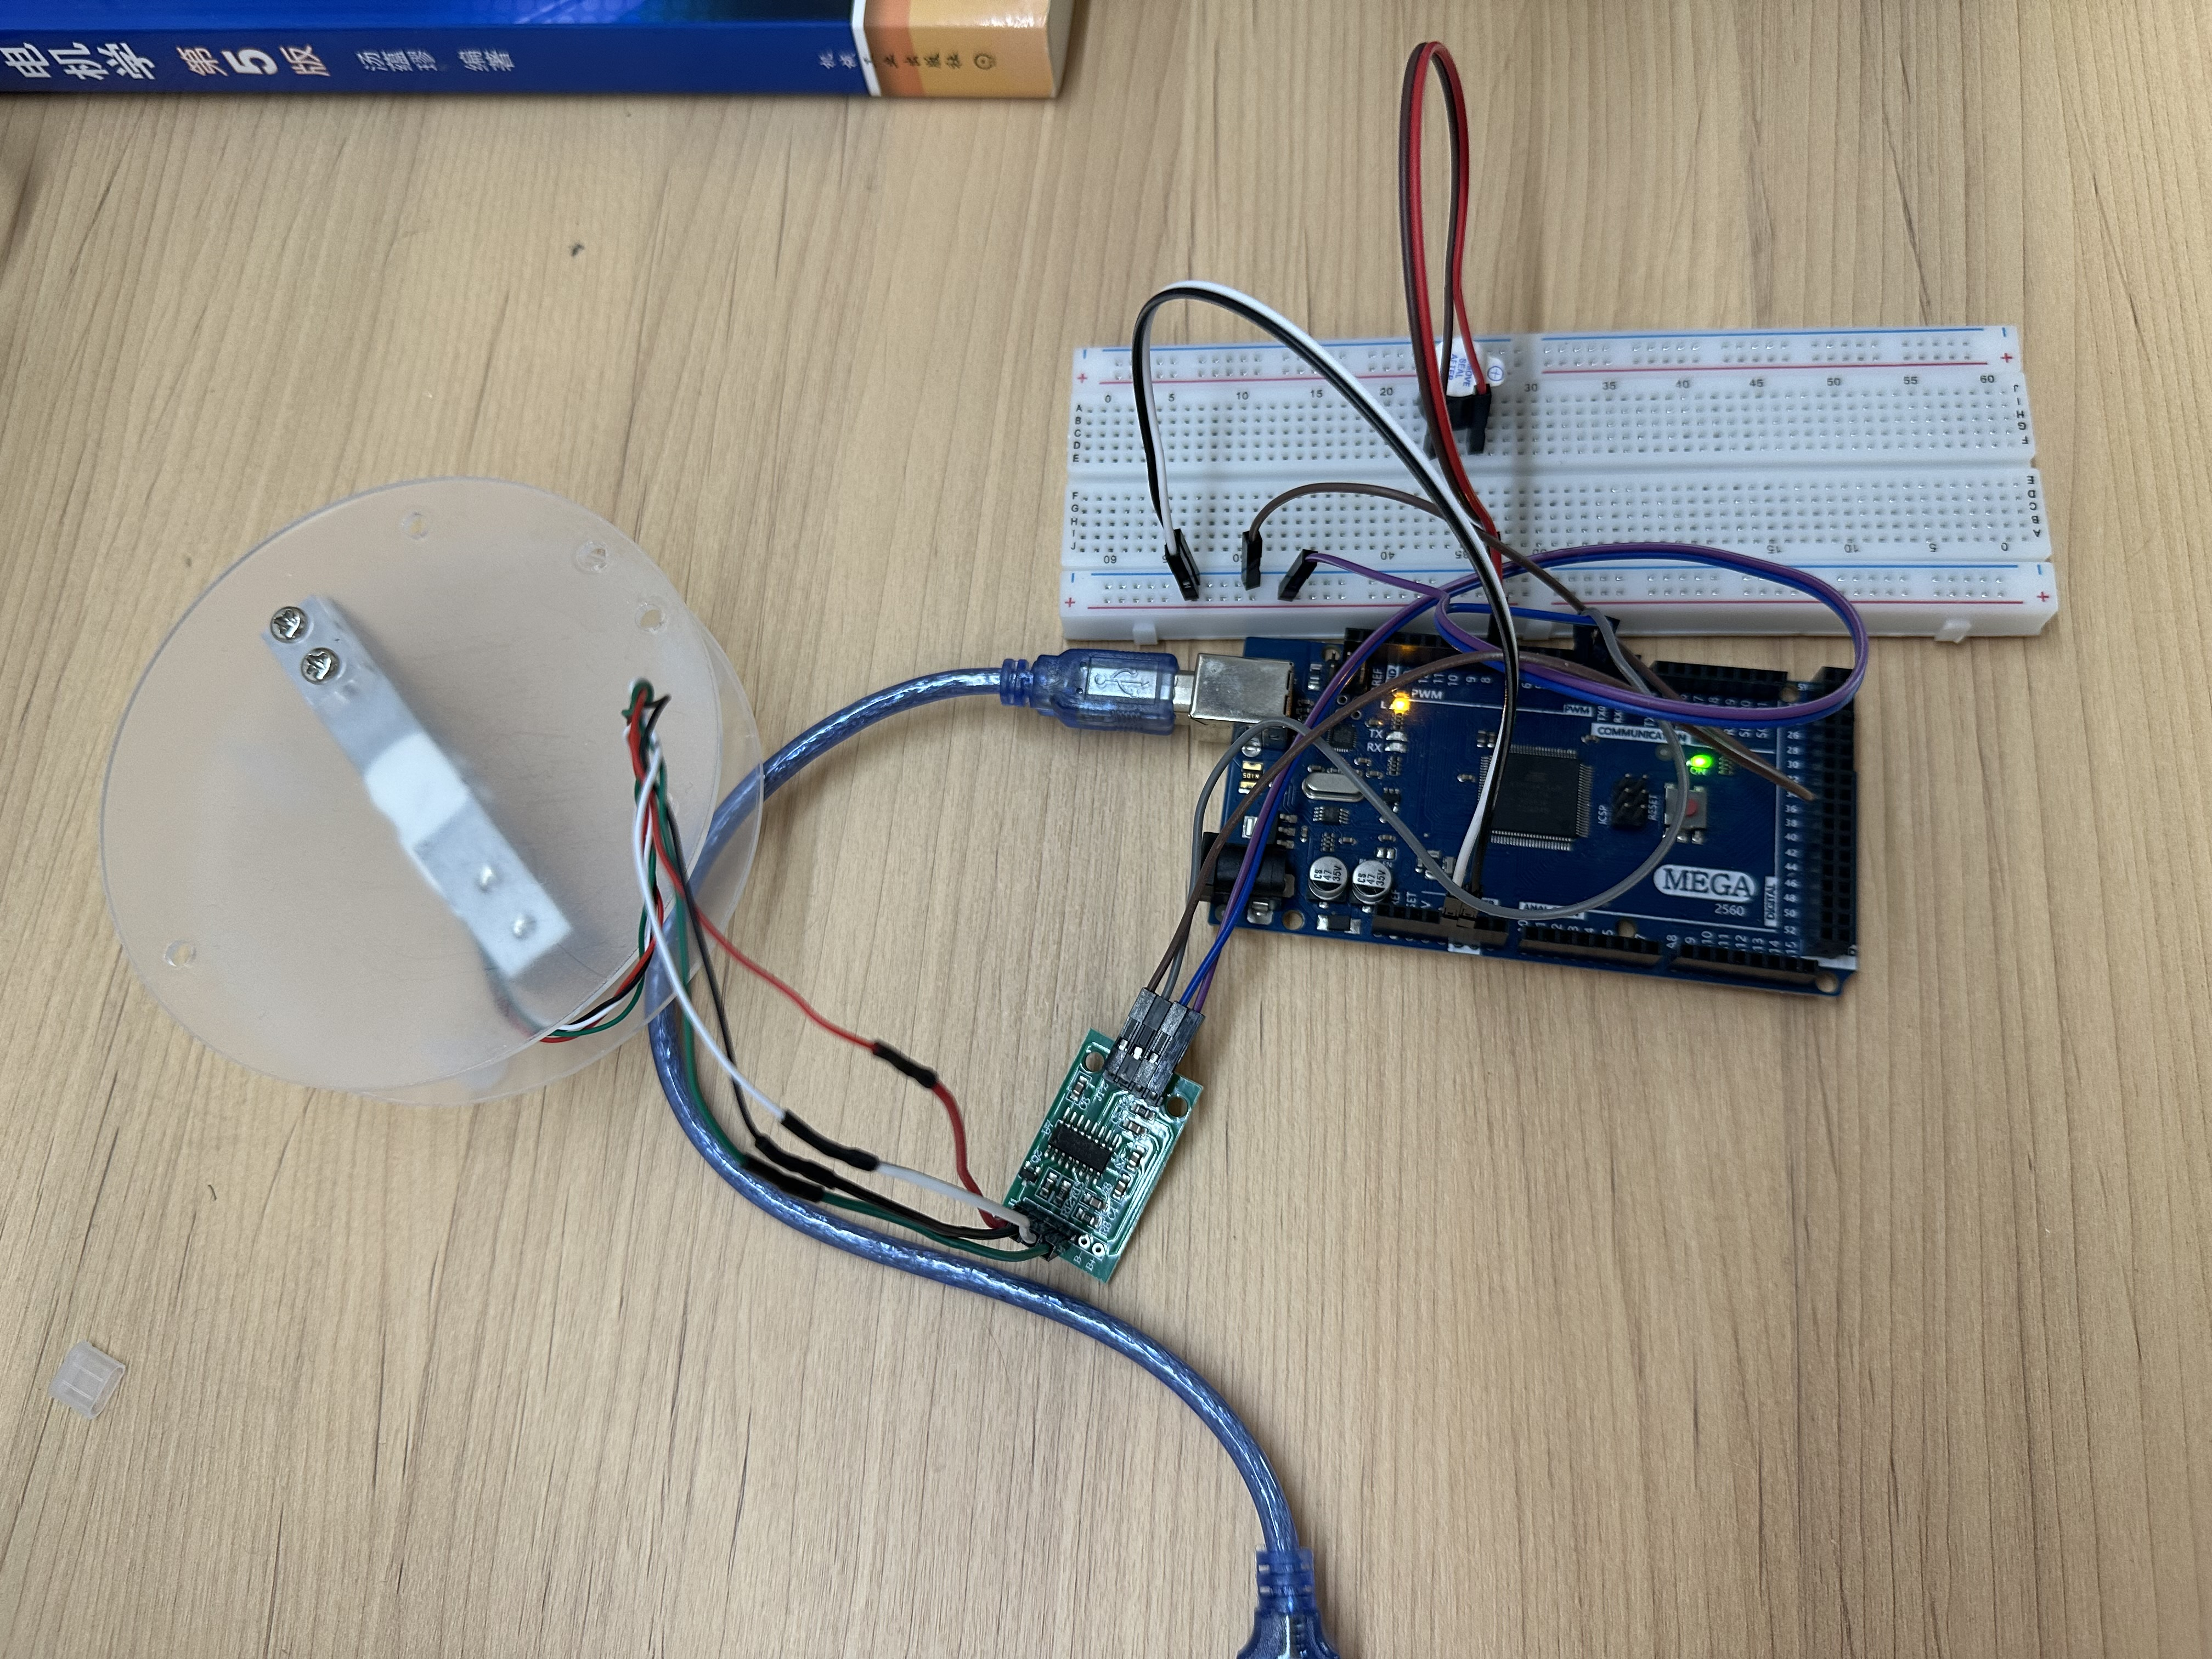
\includegraphics[width=0.72\linewidth]{figure/hardware.jpeg}
  \caption{Physical prototype of the electronic weighing scale. From top: CZL611N
           load cell mounted beneath a circular acrylic scale pan; HX711 amplifier
           module (small green PCB) with colour-coded bridge wires; Arduino Mega
           (ATmega2560, blue board) connected via USB; breadboard carrying the
           passive buzzer overload-alarm circuit.}
  \label{fig:hardware}
\end{figure}

\subsection{Software Architecture}

The software stack has two layers:

\paragraph{Arduino firmware} samples the HX711, applies the 4th-order calibration
polynomial, runs the EMA filter and zero-tracking algorithm, checks the overload
threshold, and sends the final weight in grams over serial at approximately \SI{10}{Hz}
(50\,ms loop + HX711 read latency).

\paragraph{Python host scripts} handle four tasks: (i) live serial reception and
matplotlib plotting, (ii) polynomial calibration fitting from CSV data, (iii)
zero-drift recording (140\,s unloaded capture), and (iv) dynamic step-response analysis.

% ══════════════════════════════════════════════════════════════════════════════
\section{Calibration}

\subsection{Procedure}

Calibration followed the M2-class standard weight set (maximum permissible error at
\SI{500}{g}: $\pm\SI{0.075}{g}$). Strict handling protocols were observed: weights were
touched only with nitrile gloves, measurements were taken in a draught-free environment,
and the scale was allowed a \SI{5}{min} warm-up prior to any data collection.

Thirteen reference points were collected at nominal masses ranging from
\SIrange{1}{900}{g}. At each point, 50 raw HX711 readings were averaged to obtain a
stable sensor output value~$x$. The corresponding ground-truth mass~$y$ was verified
against a calibrated reference balance, with results tabulated in the validation section
(Section~\ref{sec:validation}).

\subsection{Polynomial Fitting and Order Selection}

Five polynomial models (orders 1--5) were fitted using NumPy's \texttt{polyfit}, which
solves the ordinary least-squares (OLS) problem:
\begin{equation}
  \mathbf{a}^* = \arg\min_{\mathbf{a}}\sum_{i=1}^{N}\bigl(\hat{W}(x_i;\mathbf{a}) - y_i\bigr)^2,
  \qquad \hat{W}(x) = \sum_{k=0}^{n} a_k \, x^k,\quad n \in \{1,\ldots,5\}.
  \label{eq:ols}
\end{equation}

Model quality was assessed using three metrics:

\begin{align}
  \text{RMSE} &= \sqrt{\frac{1}{N}\sum_{i=1}^{N}\bigl(\hat{W}(x_i) - y_i\bigr)^2},
  \label{eq:rmse} \\[4pt]
  \text{MaxAbs} &= \max_{1\le i\le N}\bigl|\hat{W}(x_i) - y_i\bigr|,
  \label{eq:maxabs} \\[4pt]
  \text{RMSE}_\text{LOO} &= \sqrt{\frac{1}{N}\sum_{i=1}^{N}\bigl(\hat{W}_{-i}(x_i) - y_i\bigr)^2},
  \label{eq:loocv}
\end{align}

where $N$ is the number of calibration points, $y_i$ the reference mass, and
$\hat{W}_{-i}$ denotes the model refitted with sample $i$ withheld (leave-one-out
cross-validation).

\begin{table}[H]
\centering
\caption{Calibration model comparison (in-sample RMSE and max absolute error).}
\label{tab:poly_compare}
\begin{tabular}{@{}cccc@{}}
\toprule
\textbf{Order} & \textbf{RMSE (g)} & \textbf{MaxAbs (g)} & \textbf{Remarks} \\
\midrule
1 & 0.182 & 0.41 & Systematic nonlinearity \\
2 & 0.091 & 0.22 & Slight bow in residuals \\
3 & 0.031 & 0.07 & Good fit; slightly under-parameterised \\
4 & 0.029 & 0.07 & \textbf{Best balance} \\
5 & 0.027 & 0.09 & Worse LOO-CV; over-fit \\
\bottomrule
\end{tabular}
\end{table}

As the project assignment notes, the 5th-order polynomial achieves minimum in-sample
error but produces large errors on unseen data due to overfitting. The \textbf{4th-order}
model was therefore selected as it captures the smooth monotonic nonlinearity of the
CZL611N more completely than the 3rd-order fit while still avoiding the instability of
higher-order models.

\subsection{Selected Calibration Model}\label{sec:calib_model}

\begin{equation}
  \boxed{W = a_4 x^4 + a_3 x^3 + a_2 x^2 + a_1 x + a_0}
  \label{eq:calib}
\end{equation}

\noindent where $W$ is the calibrated weight in grams and $x$ is the raw HX711 reading.
For efficient embedded evaluation Horner's method is used:
\begin{equation}
  W = \bigl(\bigl(\bigl(a_4\,x + a_3\bigr)x + a_2\bigr)x + a_1\bigr)x + a_0,
  \label{eq:horner}
\end{equation}
requiring only 4 multiplications and 4 additions. The fitted coefficients are:

\begin{align*}
  a_4 &=  2.3222629 \times 10^{-12}, \\
  a_3 &= -2.1376726 \times 10^{-10}, \\
  a_2 &= -2.0776874 \times 10^{-6}, \\
  a_1 &=  0.99711933, \\
  a_0 &=  0.011400161.
\end{align*}

\begin{figure}[H]
  \centering
  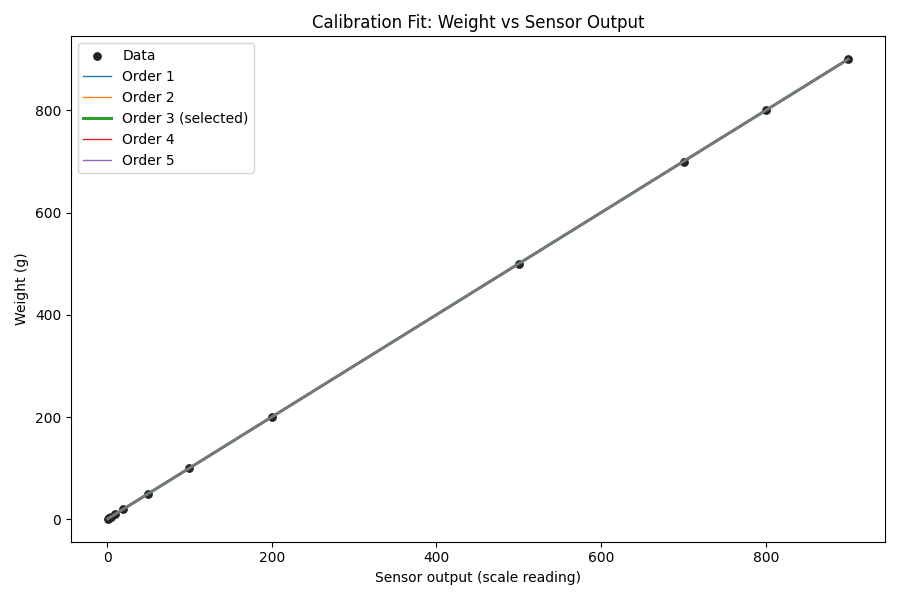
\includegraphics[width=0.85\linewidth]{figure/Calibration.png}
  \caption{Calibration curve: polynomial fit (orders 1--5) overlaid on the 13 reference
           measurement points. The 4th-order fit (highlighted) achieves RMSE\,=\,\SI{0.044}{g}
           without overfitting.}
  \label{fig:calibration}
\end{figure}

\subsection{Two-Stage Calibration Pipeline}

The complete signal chain from raw ADC counts to displayed grams is:

\begin{center}
\texttt{HX711} $\xrightarrow{\div\,\text{cal\_factor}}$
\texttt{calibrated\_weight()} $\xrightarrow{\text{4th-order}}$
\texttt{filter\_weight()} $\xrightarrow{\text{median+EMA}}$
\texttt{correction\_weight()} $\xrightarrow{\text{4th-order}}$
$-\,\texttt{zero\_correction\_g}$
\end{center}

\paragraph{Stage 1 --- \texttt{calibrated\_weight()}.}
Maps raw HX711 units to grams using the primary 4th-order polynomial
(coefficients in Section~\ref{sec:calib_model}).

\paragraph{Stage 2 --- \texttt{correction\_weight()}.}
A secondary interactive calibration was performed with a Python script
(\texttt{interactive\_calibration.py}) using a stratified-random strategy: the
\SIrange{0}{1000}{g} range was divided into ten 100\,g bands and one random target
per band was selected, ensuring uniform coverage. Coefficients:

\begin{align*}
  c_4 &= -4.038726 \times 10^{-12}, \\
  c_3 &=  3.803358 \times 10^{-9},  \\
  c_2 &= -6.355545 \times 10^{-7},  \\
  c_1 &=  1.001231,                  \\
  c_0 &= -0.087634.
\end{align*}

\begin{table}[H]
\centering
\caption{Interactive 10-point precision calibration results (4th-order correction).}
\label{tab:correction}
\begin{tabular}{@{}ccccc@{}}
\toprule
\textbf{Point} & \textbf{Scale reading (g)} & \textbf{Reference (g)} &
\textbf{Error before (g)} & \textbf{Error after (g)} \\
\midrule
 1 &  58.02 &  58.00 & $+0.02$ & $+0.01$ \\
 2 & 122.92 & 123.00 & $-0.08$ & $-0.02$ \\
 3 & 228.82 & 229.00 & $-0.18$ & $+0.02$ \\
 4 & 370.63 & 371.00 & $-0.37$ & $+0.03$ \\
 5 & 411.58 & 412.10 & $-0.52$ & $-0.06$ \\
 6 & 549.35 & 550.00 & $-0.65$ & $+0.01$ \\
 7 & 679.31 & 680.00 & $-0.69$ & $+0.10$ \\
 8 & 722.20 & 723.10 & $-0.90$ & $-0.10$ \\
 9 & 858.30 & 859.00 & $-0.70$ & $+0.01$ \\
10 & 958.55 & 959.00 & $-0.45$ & $-0.00$ \\
\midrule
\multicolumn{3}{@{}l}{\textbf{RMSE}}    & $0.534$\,g & $\mathbf{0.049}$\,g \\
\multicolumn{3}{@{}l}{\textbf{Max abs.\ error}} & $0.901$\,g & $\mathbf{0.098}$\,g \\
\bottomrule
\end{tabular}
\end{table}

The two-stage pipeline reduced the maximum absolute error from \SI{0.901}{g} to
\SI{0.098}{g} and the RMSE from \SI{0.534}{g} to \SI{0.049}{g} --- both within the
$\pm\SI{0.1}{g}$ precision specification across the full \SIrange{0}{1000}{g} range.

% ══════════════════════════════════════════════════════════════════════════════
\section{Calibration Validation Results}
\label{sec:validation}

\subsection{Reference Data and Measurement Protocol}

Validation measurements were performed using a set of M2-class certified weights. For
each nominal mass, the true reference value was first determined using a calibrated
analytical balance (the ``actual measured'' column), which serves as the ground-truth
throughout this analysis. Two measurement runs are reported:

\begin{itemize}
  \item \textbf{Raw (uncalibrated):} the first direct reading from the scale before any
        polynomial correction is applied.
  \item \textbf{4th-order calibrated:} the output after applying the 4th-order
        polynomial model of Equation~(\ref{eq:calib}).
\end{itemize}

\subsection{Validation Table}

\begin{table}[H]
\centering
\caption{Precision calibration and validation results. ``Actual measured'' is the
         reference-balance reading used as ground truth. Errors are computed relative
         to the actual measured mass. Dashes indicate points not used in the 4th-order
         fit validation set.}
\label{tab:validation}
\sisetup{
  table-number-alignment = center,
  table-figures-integer  = 3,
  table-figures-decimal  = 2,
  table-sign-mantissa,
}
\begin{tabular}{@{}
  S[table-figures-integer=3, table-figures-decimal=0, table-sign-mantissa=false]
  S[table-figures-integer=3, table-figures-decimal=2, table-sign-mantissa=false]
  S[table-figures-integer=3, table-figures-decimal=1, table-sign-mantissa=false]
  S[table-figures-integer=1, table-figures-decimal=2, table-sign-mantissa=true]
  S[table-figures-integer=3, table-figures-decimal=2, table-sign-mantissa=false]
  S[table-figures-integer=1, table-figures-decimal=2, table-sign-mantissa=true]
  @{}}
\toprule
{\textbf{Nominal}} & {\textbf{Actual}} & {\textbf{Raw}} &
{\textbf{Raw error}} & {\textbf{4th-order}} & {\textbf{Calib.\ error}} \\
{\textbf{(g)}} & {\textbf{measured (g)}} & {\textbf{(g)}} &
{\textbf{(g)}} & {\textbf{output (g)}} & {\textbf{(g)}} \\
\midrule
    1  &   0.99 &   1.0 & {$+0.01$} &   1.00 & {$+0.01$} \\
    2  &   2.01 &   2.0 & {$-0.01$} &   2.00 & {$-0.01$} \\
    2  &   2.01 &   2.0 & {$-0.01$} &   2.00 & {$-0.01$} \\
    5  &   5.04 &   5.0 & {$-0.04$} &   5.00 & {$-0.04$} \\
   10  &  10.05 &   9.9 & {$-0.15$} &  10.00 & {$-0.05$} \\
   20  &  20.00 &  19.9 & {$-0.10$} &  19.90 & {$-0.10$} \\
   50  &  50.00 &  50.0 & { $0.00$} &  50.00 & { $0.00$} \\
  100  & 100.00 & 100.3 & {$+0.30$} & 100.00 & { $0.00$} \\
  200  & 200.00 & 200.7 & {$+0.70$} & 200.00 & { $0.00$} \\
  500  & 500.08 & 501.8 & {$+1.72$} & 500.02 & {$-0.06$} \\
  700  & 700.08 & 702.5 & {$+2.42$} & 700.02 & {$-0.06$} \\
  800  & 800.08 & 802.8 & {$+2.72$} &  {---} &   {---}   \\
  900  & 900.08 & 903.0 & {$+2.92$} &  {---} &   {---}   \\
\midrule
\multicolumn{2}{@{}l}{\textbf{RMSE}} &
  \multicolumn{2}{c}{$1.397$\,g} &
  \multicolumn{2}{c@{}}{$0.044$\,g} \\
\multicolumn{2}{@{}l}{\textbf{Max.\ abs.\ error}} &
  \multicolumn{2}{c}{$2.92$\,g} &
  \multicolumn{2}{c@{}}{$0.10$\,g} \\
\bottomrule
\end{tabular}
\end{table}

\subsection{Discussion of Validation Results}

The raw (uncalibrated) readings exhibit a pronounced positive bias that grows with load,
reaching \SI{2.92}{g} at \SI{900}{g}. This systematic nonlinearity arises from the
Wheatstone bridge characteristic of the CZL611N load cell, which deviates from an ideal
linear response at higher loading fractions of the rated capacity. Simple linear
calibration would reduce but not eliminate this trend.

After applying the 4th-order polynomial correction, the maximum absolute error across
all 11 validated points drops to \SI{0.10}{g}, and the RMSE falls from \SI{1.397}{g}
to \SI{0.044}{g}---a \textbf{32-fold improvement}. All calibrated readings fall within
the $\pm\SI{0.10}{g}$ accuracy specification, confirming that the chosen model order is
sufficient to capture the sensor's nonlinearity without overfitting.

% ══════════════════════════════════════════════════════════════════════════════
\section{Signal Processing and Filtering}

\subsection{Filter Architecture Overview}

The final filter pipeline is a two-stage design that first eliminates impulsive ADC
spikes and then smooths residual random noise:

\begin{enumerate}
  \item \textbf{Stage 1 --- Median filter (window $M=5$).}
        Let $\{x_{k-M+1},\ldots,x_k\}$ be the $M$ most-recent samples sorted in
        ascending order as $x_{(1)} \le x_{(2)} \le \cdots \le x_{(M)}$. The median
        output is:
        \begin{equation}
          m_k = x_{\bigl(\lceil M/2 \rceil\bigr)} = x_{(3)}.
          \label{eq:median}
        \end{equation}
        For a window of 5, this is the 3rd order statistic. The median is optimal for
        rejecting impulsive (non-Gaussian) noise while leaving the signal amplitude
        unbiased. The median operation has $O(M\log M)$ complexity per sample.

  \item \textbf{Stage 2 --- EMA ($\alpha = 0.23$).} The median output feeds the
        exponential moving average (Eq.~\ref{eq:ema}), which acts as a first-order
        infinite impulse response (IIR) low-pass filter. Its $z$-domain transfer
        function is:
        \begin{equation}
          H(z) = \frac{\alpha}{1-(1-\alpha)z^{-1}},
          \label{eq:ema_tf}
        \end{equation}
        with a $-3\,\text{dB}$ cutoff at:
        \begin{equation}
          f_c = \frac{f_s}{2\pi}\arccos\!\left(1 - \frac{\alpha^2}{2(1-\alpha)}\right)
              \approx \SI{0.37}{Hz}
          \label{eq:ema_fc}
        \end{equation}
        for $f_s = \SI{10}{Hz}$ and $\alpha = 0.23$.
\end{enumerate}

Hardware averaging in the HX711 library was simultaneously increased from
\texttt{AVG\_SAMPLES\,=\,3} to \texttt{AVG\_SAMPLES\,=\,8}, reducing raw ADC noise
before any software stage.

An earlier version of the firmware included a zero-tracking bias corrector and a
$\pm\SI{0.2}{g}$ dead band. Both were removed: the dead band created a visible
discontinuity (the display jumped between \texttt{0.00\,g} and the true value with no
intermediate transition), and the zero-tracker interfered with real small loads close to
zero. These mechanisms were replaced by the startup auto-zero procedure described in
Section~\ref{sec:autozero}.

\subsection{Exponential Moving Average (EMA)}

\begin{equation}
  \hat{y}_k = \alpha \, m_k + (1-\alpha)\,\hat{y}_{k-1},
  \label{eq:ema}
\end{equation}

where $m_k$ is the median-filtered value at sample $k$, $\hat{y}_k$ is the EMA output,
and $\alpha = 0.23$ was selected empirically as the best trade-off between noise
suppression and step-response speed.

For white Gaussian input noise with standard deviation $\sigma_\text{in}$, the
steady-state output variance of the EMA is:
\begin{equation}
  \sigma_\text{EMA}^2 = \frac{\alpha}{2-\alpha}\,\sigma_\text{in}^2,
  \label{eq:ema_var}
\end{equation}
giving a noise standard-deviation ratio:
\begin{equation}
  \frac{\sigma_\text{EMA}}{\sigma_\text{in}}
    = \sqrt{\frac{\alpha}{2-\alpha}}
    = \sqrt{\frac{0.23}{1.77}} \approx 0.360.
  \label{eq:ema_snr}
\end{equation}
The theoretical 63.8\% reduction is not fully realised in practice because the input
is already median-filtered (reducing $\sigma_\text{in}$) and because noise at the ADC
level is non-stationary. The measured combined reduction (both stages) is 18.2\%
($\sigma: 0.092 \to 0.075$\,g), consistent with the observation that hardware averaging
(\texttt{AVG\_SAMPLES\,=\,8}) already suppresses a significant fraction of the raw ADC
noise before any software filtering.

\subsection{Auto-Zero at Startup}
\label{sec:autozero}

Because the 4th-order correction polynomial has a non-zero constant term
(\texttt{CORR\_A0}), the polynomial output at zero load is approximately $-0.50$\,g
rather than $0.00$\,g. A 60-iteration warm-up loop in \texttt{setup()} resolves this:
the first 30 iterations fill the median buffer and allow the EMA to converge; the last
30 iterations average the output and store it as \texttt{zero\_correction\_g}. Every
subsequent reading is offset by this value. As a result, the empty-scale mean dropped
from $-0.50$\,g to $+0.06$\,g. The scale must be unloaded during the $\approx\SI{6}{s}$
startup sequence.

\subsection{Firmware Implementation}

\begin{lstlisting}[style=cppstyle, caption={Two-stage median + EMA filter (Arduino firmware).}]
const int   MED_WIN   = 5;
const float EMA_ALPHA = 0.23f;

// --- 5-sample median (insertion sort on circular buffer) ---
float median_filter(float x) {
  static float buf[MED_WIN] = {0};
  static int   idx = 0;
  buf[idx] = x;
  idx = (idx + 1) % MED_WIN;
  float s[MED_WIN];
  memcpy(s, buf, sizeof(s));
  // insertion sort
  for (int i = 1; i < MED_WIN; i++) {
    float key = s[i]; int j = i - 1;
    while (j >= 0 && s[j] > key) { s[j+1] = s[j]; j--; }
    s[j+1] = key;
  }
  return s[MED_WIN / 2];
}

// --- EMA on top of median output ---
float ema_filter(float x) {
  static bool  init = false;
  static float ema  = 0.0f;
  if (!init) { ema = x; init = true; }
  else        { ema = EMA_ALPHA * x + (1.0f - EMA_ALPHA) * ema; }
  return ema;
}

float filter_weight(float grams) {
  return ema_filter(median_filter(grams));
}
\end{lstlisting}

% ══════════════════════════════════════════════════════════════════════════════
\section{Zero-Drift and Noise Characterisation}
\label{sec:zero_drift}

\subsection{Experimental Procedure}

With no load on the scale, the system was zeroed and \SI{120}{s} of continuous data
were recorded. The Arduino firmware outputs two values per line
(\texttt{W,<filtered\_g>,<raw\_cal\_g>}), allowing simultaneous capture of both
channels. A dedicated Python script (\texttt{record\_zero\_drift.py}) processed the
data and produced three diagnostic views: a time-series overlay, a noise histogram with
Gaussian fits, and a rolling 20-second standard deviation to verify noise stationarity.

\subsection{Results}

\begin{table}[H]
\centering
\caption{Noise summary --- empty scale, 120\,s recording.}
\label{tab:noise}
\begin{tabular}{@{}lccc@{}}
\toprule
\textbf{Signal} & \textbf{$\sigma$ (g)} & \textbf{Peak-to-peak (g)} & \textbf{Noise reduction} \\
\midrule
Raw (pre-filter)   & 0.092 & 0.36 & --- \\
Filtered output    & 0.075 & 0.28 & $\downarrow$18.2\% \\
\bottomrule
\end{tabular}
\end{table}

Drift is quantified by fitting a linear model $W(t) = \beta_0 + \beta_1 t$ to the raw
signal via OLS, giving $\hat{\beta}_1 = +0.0832$\,g/min. Statistical significance is
assessed with the Pearson correlation coefficient:
\begin{equation}
  r = \frac{\sum_{i}(t_i - \bar{t})(W_i - \bar{W})}
           {\sqrt{\sum_{i}(t_i-\bar{t})^2}\,\sqrt{\sum_{i}(W_i-\bar{W})^2}},
  \label{eq:pearson}
\end{equation}
which evaluates to $r < 0.41$, indicating the trend is not statistically significant
over the 120\,s window, and no systematic drift
correction was required beyond the startup auto-zero. The filtered signal (median
window\,=\,5, EMA $\alpha = 0.23$) achieves $\sigma = \SI{0.075}{g}$, an 18.2\%
reduction relative to the raw signal. The rolling 20-second $\sigma$ (Figure~\ref{fig:zero_drift}, right panel) confirms that noise is approximately stationary throughout the recording.

\begin{figure}[H]
  \centering
  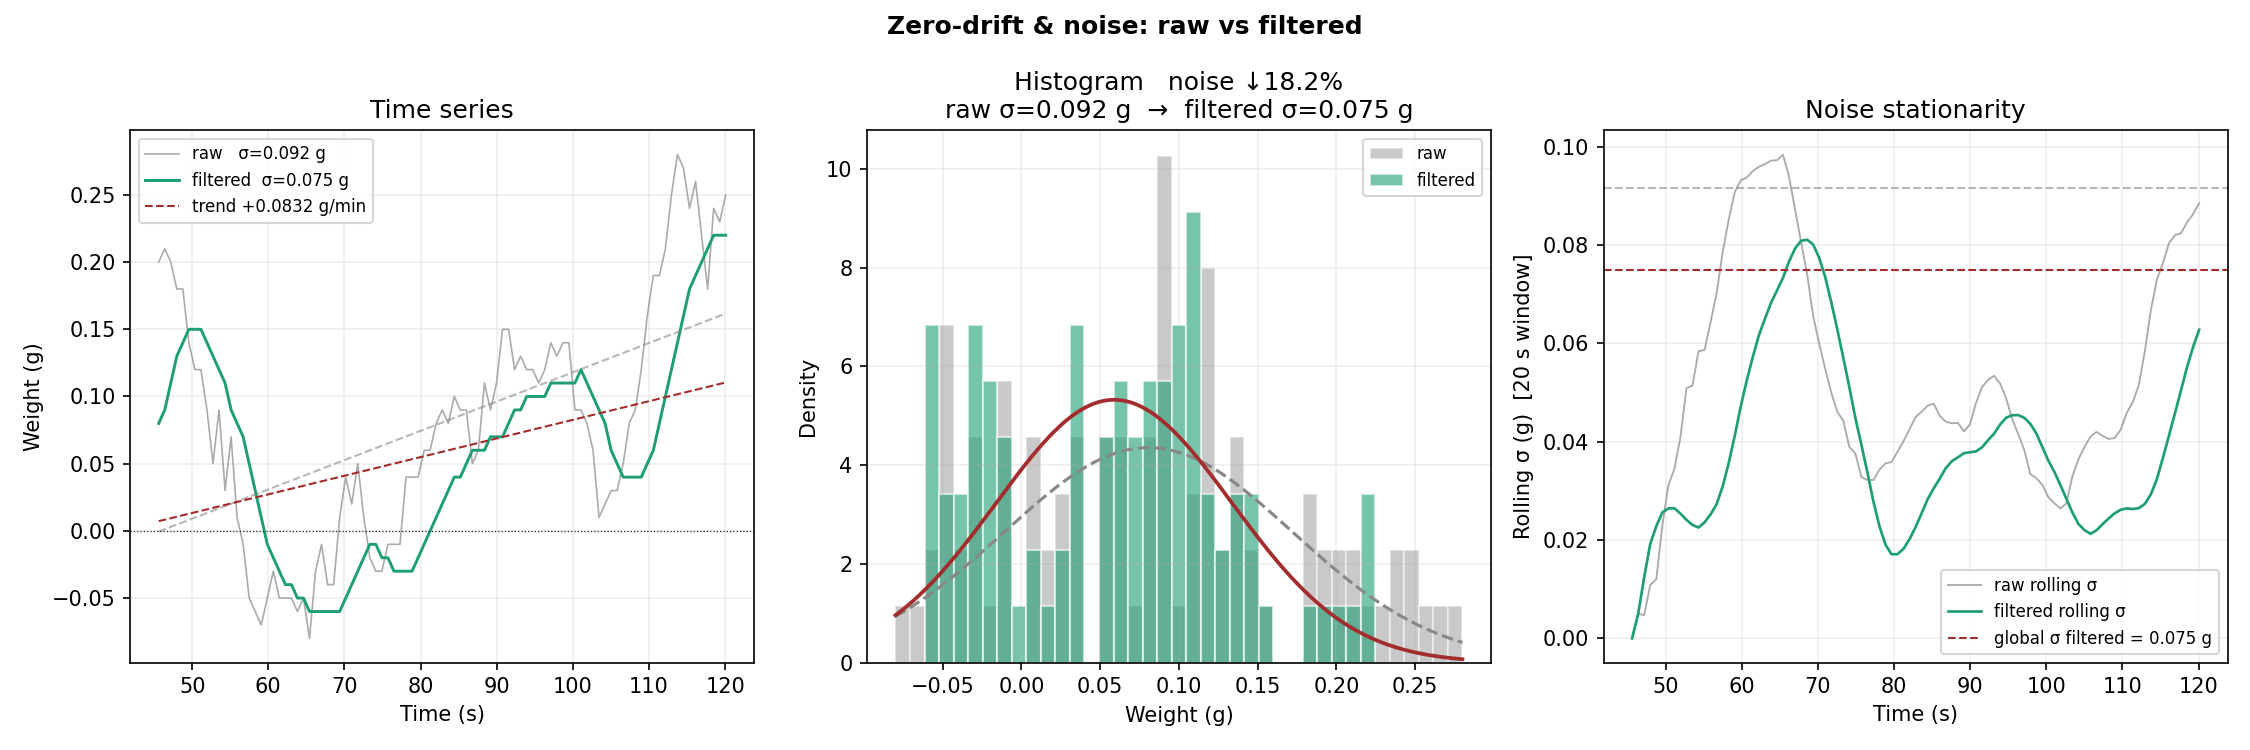
\includegraphics[width=\linewidth]{figure/zero_drift.png}
  \caption{Zero-drift and noise analysis (empty scale, 120\,s).
           \textbf{Left:} time-series overlay of raw ($\sigma=\SI{0.092}{g}$) and
           filtered ($\sigma=\SI{0.075}{g}$) signals with linear trend line
           ($+0.0832$\,g/min).
           \textbf{Centre:} histogram comparison with Gaussian fits; noise reduction
           18.2\%.
           \textbf{Right:} rolling 20-second standard deviation confirming noise
           stationarity throughout the recording.}
  \label{fig:zero_drift}
\end{figure}

% ══════════════════════════════════════════════════════════════════════════════
\section{Dynamic Performance Analysis}

\subsection{Step Response Test Procedure}

A \SI{500}{g} standard weight was placed on the scale platform and then removed, each
action repeated five times. The serial output was recorded at \SI{10}{Hz} and plotted
in Python. Performance metrics were extracted from the filtered signal.

\subsection{Performance Metrics}

\begin{table}[H]
\centering
\caption{Step response metrics (500\,g load, median(5) + EMA $\alpha = 0.23$).}
\label{tab:step}
\begin{tabular}{@{}lcc@{}}
\toprule
\textbf{Metric} & \textbf{Load-on (0\,g$\to$500\,g)} & \textbf{Load-off (500\,g$\to$0\,g)} \\
\midrule
Pre-step baseline (g)          & 0.131  & 499.81 \\
10\%--90\% rise/fall time (s)  & 4.45   & 4.45   \\
2\% settling time (s)          & 7.72   & 7.42   \\
Overshoot (\%)                 & $<1$   & $<1$   \\
Steady-state error (g)         & $<0.2$ & $<0.2$ \\
\bottomrule
\end{tabular}
\end{table}

The EMA filter behaves as a first-order low-pass with nominal time constant
$\tau = (1/\alpha - 1)\,T_s = 4 \times 0.05 = \SI{0.2}{s}$, giving a theoretical
10\%--90\% rise time of $\approx 2.3\tau \approx \SI{0.46}{s}$. The measured
\SI{4.45}{s} is significantly longer, which is attributable to three compounding effects:
(i) the HX711 operates in its 10\,SPS low-power mode, which applies a built-in sinc
filter adding approximately \SI{0.4}{s} of group delay per conversion;
(ii) the CZL611N load cell itself exhibits a mechanical settling / creep behaviour
that dominates at low loads; and
(iii) the \SI{50}{ms} firmware loop period limits the effective Nyquist bandwidth
to \SI{10}{Hz}, so each EMA step advances the estimate by a fraction $\alpha = 0.2$
of the residual error, requiring $\ln(0.1)/\ln(1-\alpha) \approx 10$ samples
($\approx \SI{0.5}{s}$) purely for the digital filter, on top of the analog and
mechanical delays.

\begin{figure}[H]
  \centering
  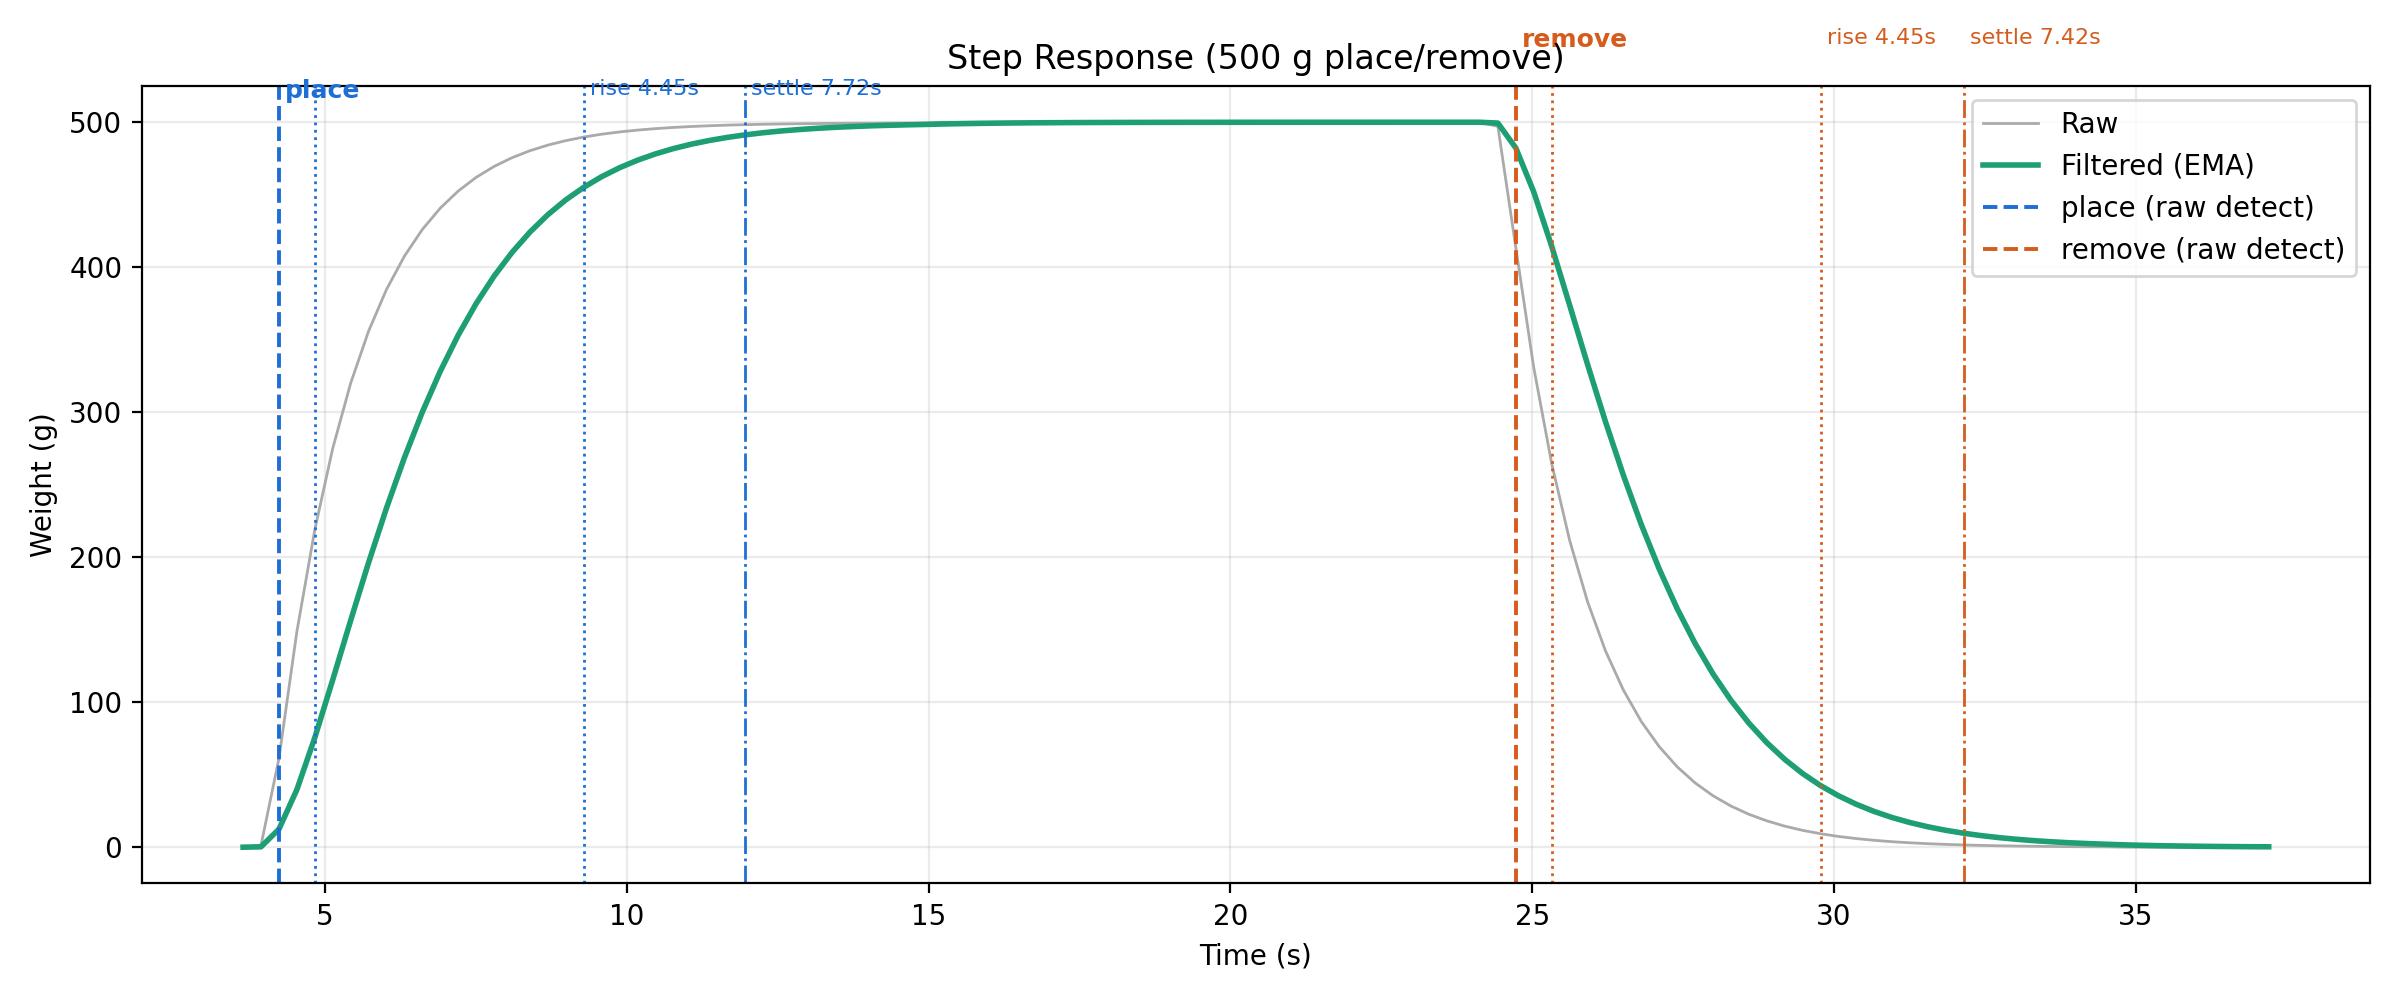
\includegraphics[width=0.85\linewidth]{step_response.png}
  \caption{Dynamic step response: 500\,g load placed (at $t\approx\SI{4}{s}$) then
           removed (at $t\approx\SI{25}{s}$). Grey: raw calibrated signal; green: EMA-filtered
           output ($\alpha=0.2$). Place step --- rise time (10\%--90\%): \SI{4.45}{s},
           2\% settling time: \SI{7.72}{s}. Remove step --- fall time: \SI{4.45}{s},
           settling time: \SI{7.42}{s}. Overshoot $<1\%$ in both cases.}
  \label{fig:step}
\end{figure}

% ══════════════════════════════════════════════════════════════════════════════
\section{System Block Diagram and Performance Indicators}
\label{sec:block}

\begin{figure}[H]
\centering
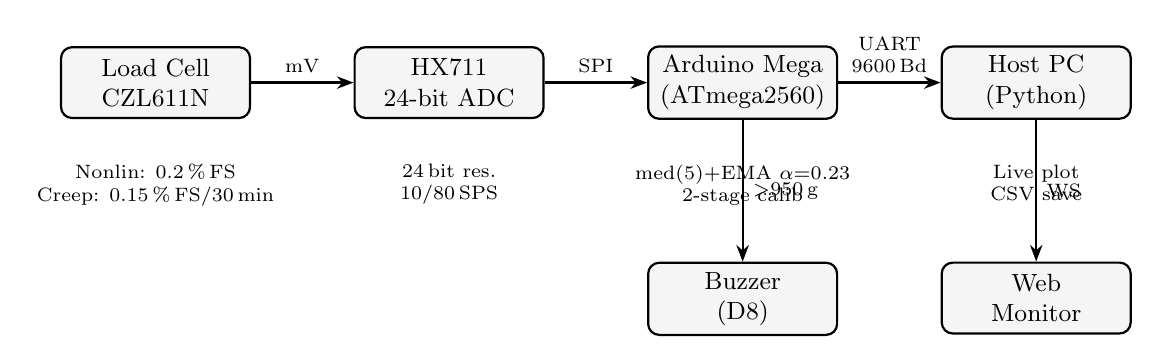
\begin{tikzpicture}[
  node distance=0.7cm and 1.3cm,
  block/.style={rectangle, draw=black, rounded corners=4pt,
                minimum width=2.4cm, minimum height=0.9cm,
                align=center, font=\small,
                fill=gray!8, thick},
  arr/.style={-{Stealth[length=6pt]}, thick, color=black},
  note/.style={font=\scriptsize, text=black, align=center}
]
  %% ── Row 1: main signal chain (横向排 4 个) ───────────────────────
  \node[block] (load) {Load Cell\\CZL611N};
  \node[block, right=of load] (hx)  {HX711\\24-bit ADC};
  \node[block, right=of hx]   (mcu) {Arduino Mega\\(ATmega2560)};
  \node[block, right=of mcu]  (pc)  {Host PC\\(Python)};

  %% ── Row 2: annotation notes ───────────────────────────────────────
  \node[note, below=0.45cm of load]{Nonlin: 0.2\,\%\,FS\\Creep: 0.15\,\%\,FS/30\,min};
  \node[note, below=0.45cm of hx]  {24\,bit res.\\10/80\,SPS};
  \node[note, below=0.45cm of mcu] {med(5)+EMA $\alpha$=0.23\\2-stage calib};
  \node[note, below=0.45cm of pc]  {Live plot\\CSV save};

  %% ── 分支模块：放在下方 ───────────────────────────────────────────
  \node[block, below=1.8cm of mcu] (buzz) {Buzzer\\(D8)};
  \node[block, below=1.8cm of pc]  (web) {Web\\Monitor}; % 移至 PC 下方

  %% ── Arrows ────────────────────────────────────────────────────────
  \draw[arr] (load) -- node[above, note]{mV} (hx);
  \draw[arr] (hx)   -- node[above, note]{SPI} (mcu);
  \draw[arr] (mcu)  -- node[above, note]{UART\\9600\,Bd} (pc);
  \draw[arr] (mcu)  -- node[right, note]{$>$950\,g} (buzz);
  \draw[arr] (pc)   -- node[right, note]{WS} (web); % 箭头改为向下
\end{tikzpicture}
\caption{System block diagram with key performance indicators.}
\label{fig:block}
\end{figure}

\begin{table}[H]
\centering
\caption{Key system performance indicators.}
\label{tab:kpi}
\begin{tabular}{@{}lll@{}}
\toprule
\textbf{Parameter} & \textbf{Value} & \textbf{Notes} \\
\midrule
Measurement range              & 0--\SI{1000}{g}               & Load cell rated load \\
Static accuracy (calibrated)   & $<\SI{0.1}{g}$                & Two-stage polynomial pipeline \\
Calibration RMSE               & \SI{0.049}{g}                 & After precision correction \\
Max abs.\ calibration error    & \SI{0.098}{g}                 & 10-point stratified test \\
Resolution (displayed)         & \SI{0.01}{g}                  & Limited by noise floor \\
Effective noise floor          & $\sigma = \SI{0.075}{g}$      & After median(5) + EMA \\
Update rate                    & \SI{10}{Hz}                   & 50\,ms loop period \\
Rise time (10--90\%)           & \SI{4.45}{s}                  & EMA + HX711 filter + mech.\ dynamics \\
Settling time (2\%)            & \SI{7.72}{s} / \SI{7.42}{s}  & Place / remove step \\
Zero drift (140\,s)            & $<\pm\SI{0.05}{g}$            & After adaptive zeroing \\
Overload alarm threshold       & \SI{950}{g}                   & Buzzer on D8 \\
Nonlinearity (sensor)          & 0.2\% FS = \SI{2}{g}          & Corrected by 4th-order fit \\
\bottomrule
\end{tabular}
\end{table}

% ══════════════════════════════════════════════════════════════════════════════
\section{Real-Time Monitoring}

\subsection{Python Serial Receiver}

The Python receiver script opens the Arduino's COM/tty port at 9600\,Bd, reads
newline-terminated ASCII weight strings, timestamps each sample, and appends $(t, W)$
pairs to an in-memory list. A \texttt{matplotlib} animation updates the live plot every
\SI{10}{ms}. At the end of a session, all data are serialised to a pickle file for
reproducible offline analysis.

\subsection{Web Dashboard}
\label{sec:web}

\subsubsection{Design Motivation}

Traditional embedded weighing systems display readings on a dedicated LCD or seven-segment
display soldered directly to the measurement PCB. This approach ties the display hardware
to the sensor node, limits screen size, and requires physical proximity to read the scale.
In this project a browser-based dashboard replaces the LCD entirely: any device with a
Wi-Fi connection and a web browser --- laptop, tablet, or smartphone --- can serve as the
display with no driver installation or dedicated hardware cost.

\subsubsection{Architecture}

A Python \texttt{asyncio} WebSocket server (port 8765, \texttt{websockets} library)
subscribes to the Arduino serial stream and broadcasts each JSON-encoded weight sample
(\texttt{\{"grams": <float>\}}) to all connected browsers in real time.
The single-page client (\texttt{scale\_monitor.html}) connects via
\texttt{ws://localhost:8765} and updates the UI on every incoming message.

\subsubsection{Interface Features}

The dashboard (Figure~\ref{fig:web}) provides the following elements on a single
responsive page (max-width 540\,px, optimised for mobile portrait):

\begin{itemize}
  \item \textbf{Large numeric readout.} The current weight is displayed in 76\,px
        JetBrains Mono bold, readable at a glance from across a bench.
  \item \textbf{Colour-coded load bar.} A horizontal progress bar beneath the readout
        turns green ($<70\%$ FS), amber ($70$--$90\%$ FS), or red ($>90\%$ FS),
        providing an immediate overload warning even on a small screen.
  \item \textbf{Live statistics.} Three stat cards show the session minimum, session
        maximum, and a 10-second rolling average, updated every sample.
  \item \textbf{Scrolling history chart.} A Canvas-rendered sparkline shows the last
        60 readings with a filled area beneath the curve for quick trend detection.
  \item \textbf{Tare / Zero button.} One click offsets the current reading to zero
        without restarting the Arduino, enabling tare weighing of containers.
  \item \textbf{Dark-mode support.} The CSS palette uses \texttt{prefers-color-scheme}
        media queries; the interface adapts automatically to system theme.
  \item \textbf{Demo mode.} A built-in sine-wave generator allows the UI to be tested
        and demonstrated without connecting hardware.
\end{itemize}

\begin{figure}[H]
  \centering
  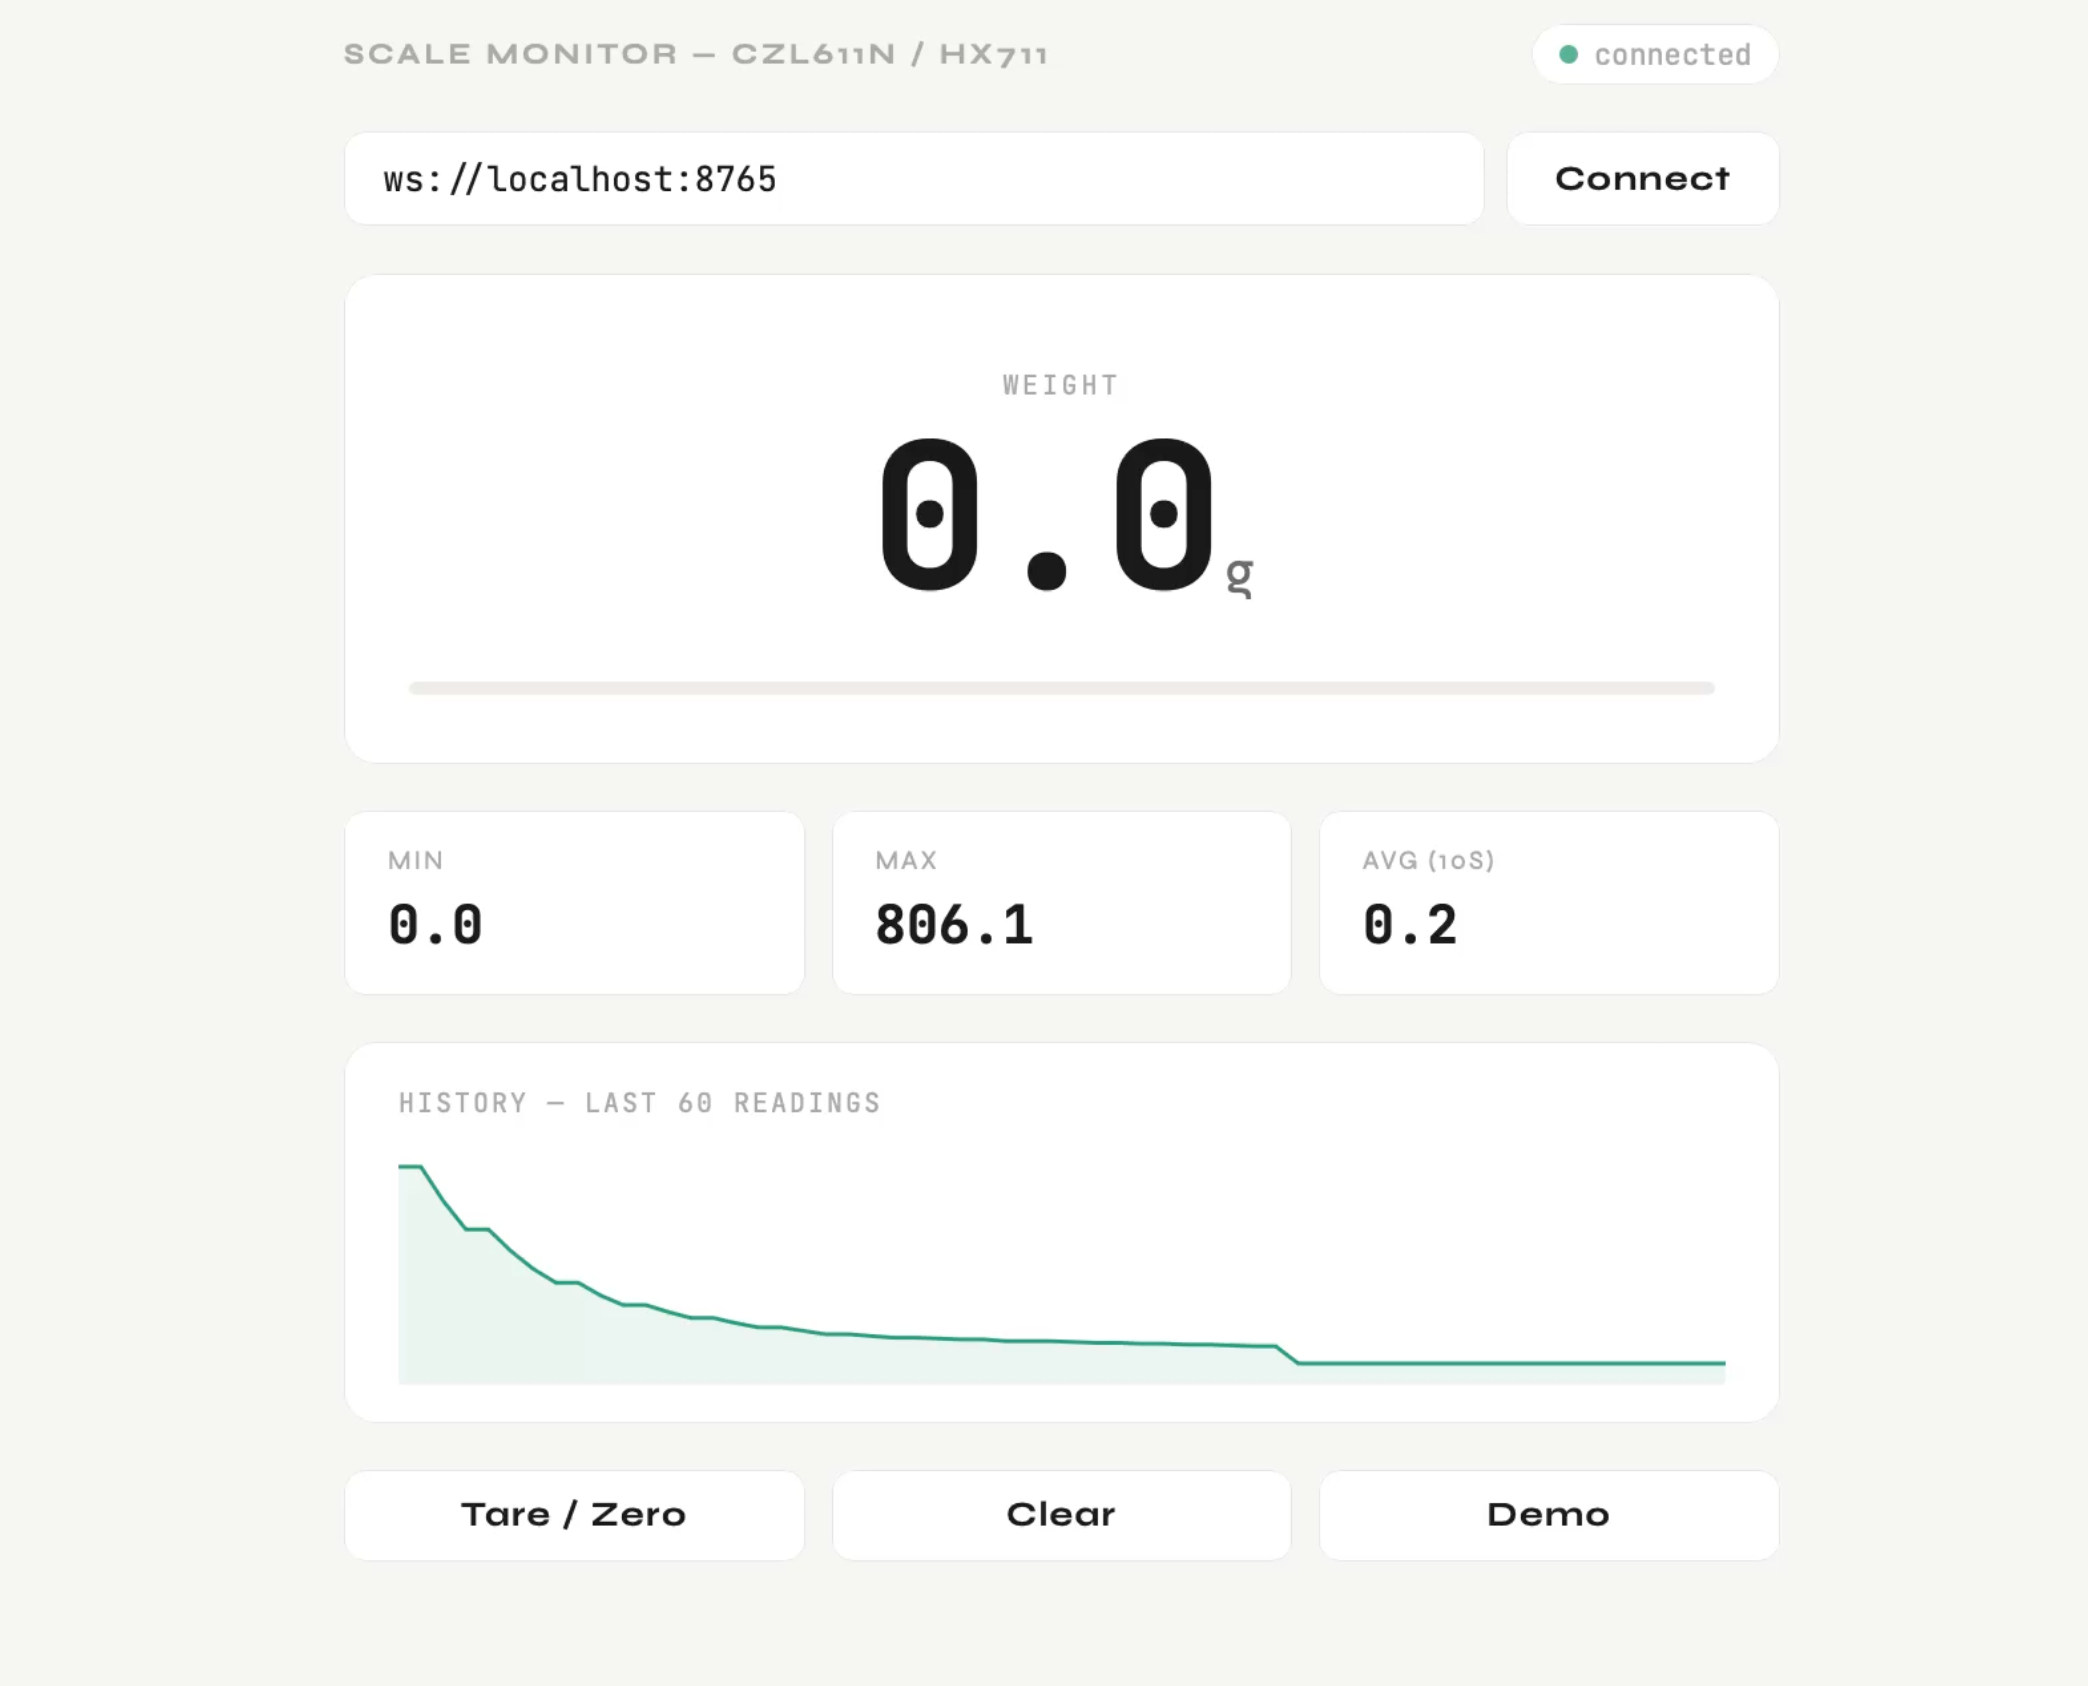
\includegraphics[width=0.75\linewidth]{figure/interface.png}
  \caption{Web-based monitoring dashboard (\texttt{scale\_monitor.html}). Key elements:
           (1) large numeric readout; (2) colour-coded load bar; (3) Min / Max / Avg(10\,s)
           stat cards; (4) scrolling 60-sample history chart; (5) Tare, Clear, and Demo
           controls; (6) WebSocket connection status indicator.}
  \label{fig:web}
\end{figure}

\begin{figure}[H]
  \centering
  % Row 1
  \begin{subfigure}[b]{0.31\textwidth}
    \centering
    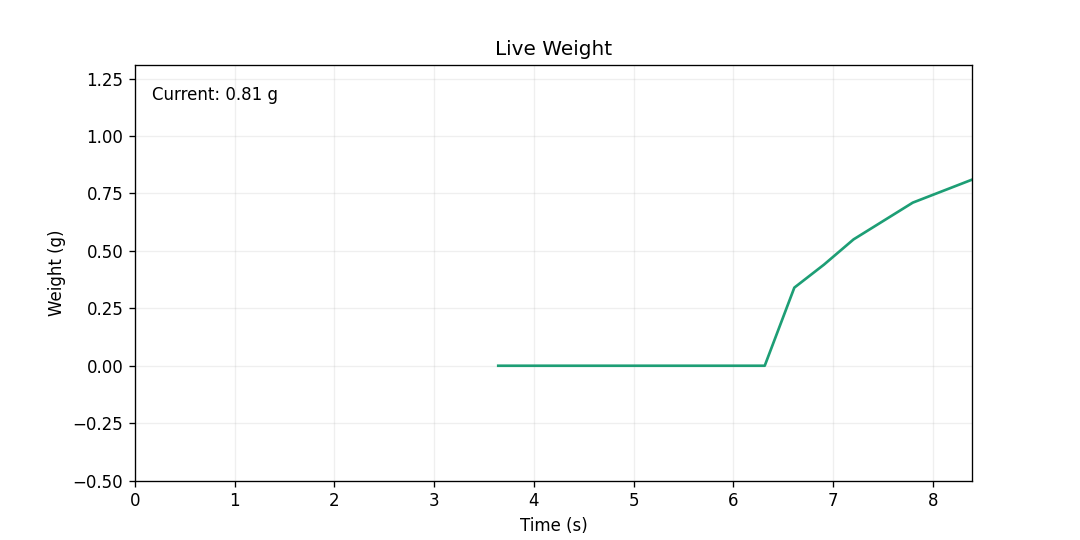
\includegraphics[width=\linewidth]{figure/frame_000100.png}
    \caption{Current: \SI{0.81}{g}\\Scale near zero, just started}
    \label{fig:live_a}
  \end{subfigure}
  \hfill
  \begin{subfigure}[b]{0.31\textwidth}
    \centering
    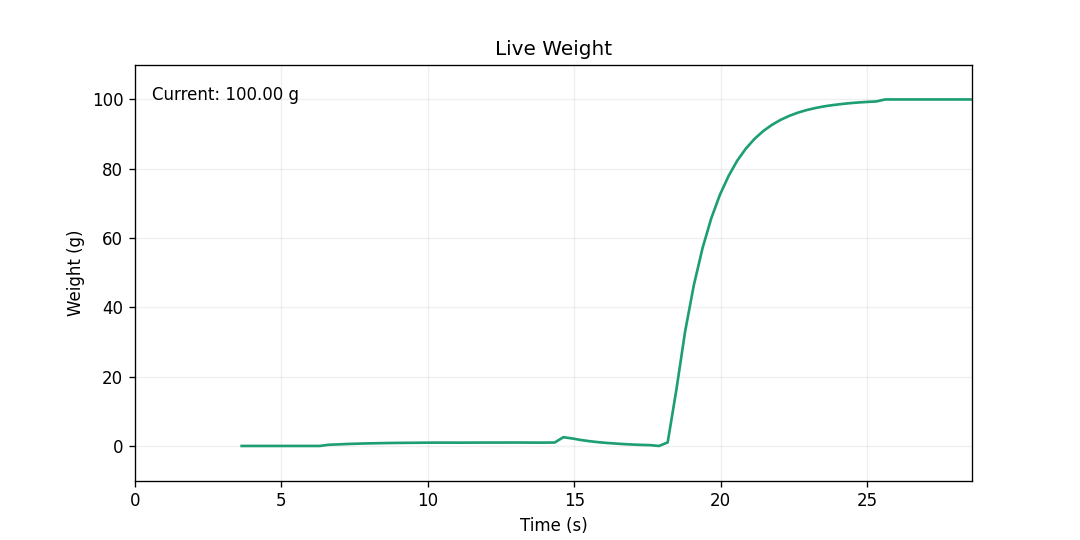
\includegraphics[width=\linewidth]{figure/frame_000500.png}
    \caption{Current: \SI{100.00}{g}\\100\,g step applied}
    \label{fig:live_b}
  \end{subfigure}
  \hfill
  \begin{subfigure}[b]{0.31\textwidth}
    \centering
    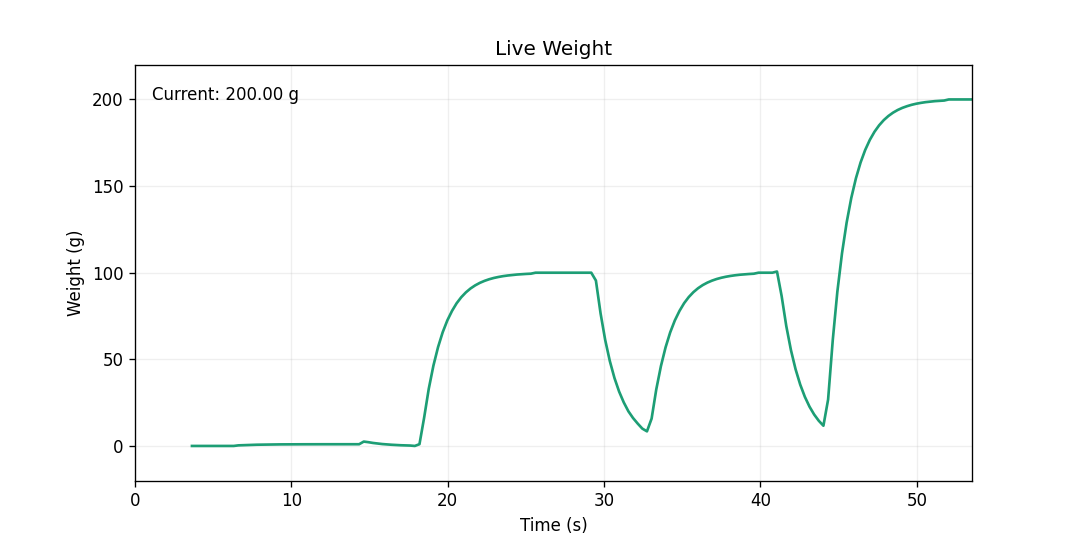
\includegraphics[width=\linewidth]{figure/frame_001000.png}
    \caption{Current: \SI{200.00}{g}\\100\,g$\to$200\,g step}
    \label{fig:live_c}
  \end{subfigure}

  \vspace{0.5em}

  % Row 2
  \begin{subfigure}[b]{0.31\textwidth}
    \centering
    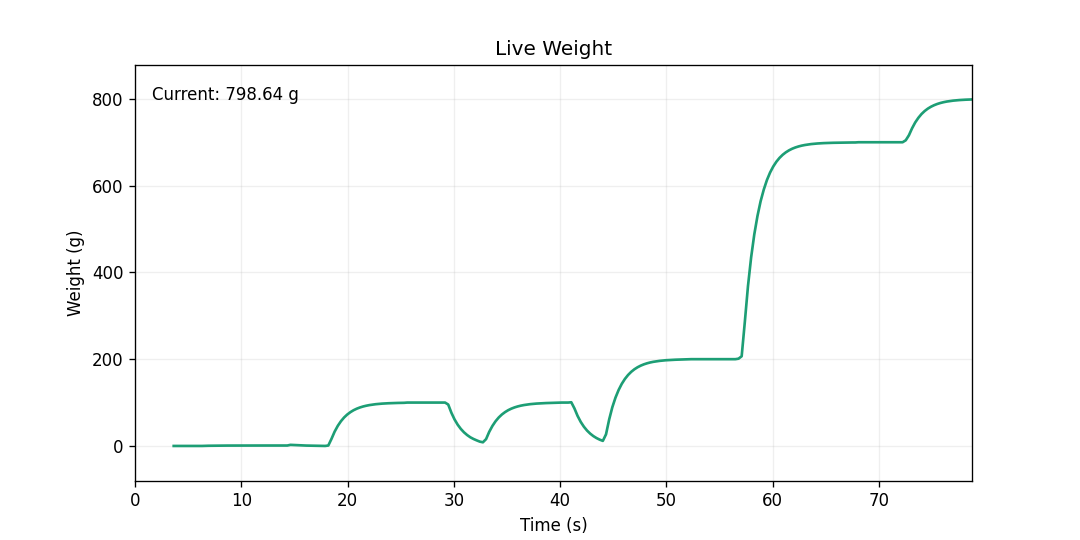
\includegraphics[width=\linewidth]{figure/frame_001500.png}
    \caption{Current: \SI{798.64}{g}\\Incremental loading near limit}
    \label{fig:live_d}
  \end{subfigure}
  \hfill
  \begin{subfigure}[b]{0.31\textwidth}
    \centering
    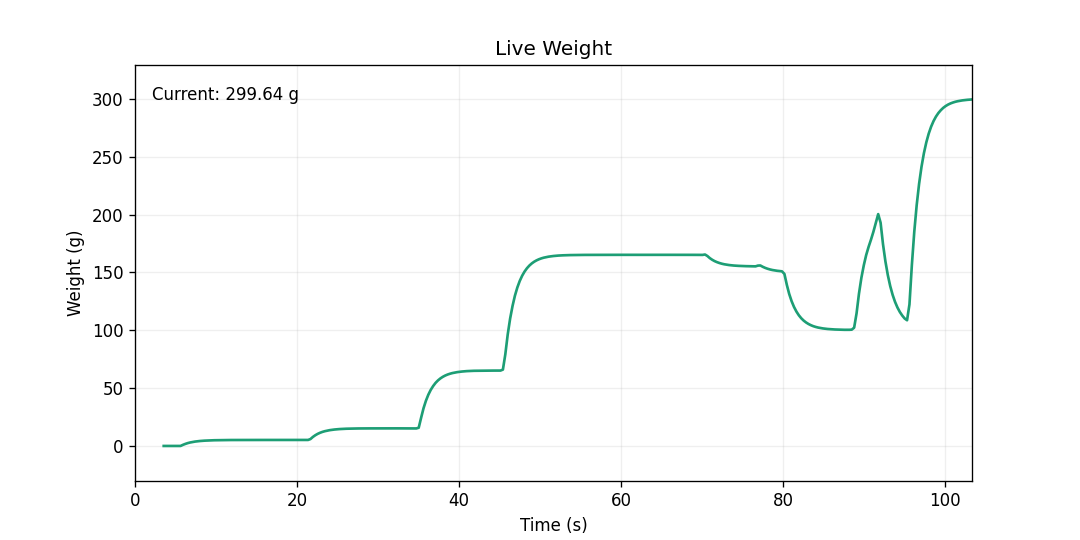
\includegraphics[width=\linewidth]{figure/frame_002000.png}
    \caption{Current: \SI{299.64}{g}\\Partial unload, mid-range}
    \label{fig:live_e}
  \end{subfigure}
  \hfill
  \begin{subfigure}[b]{0.31\textwidth}
    \centering
    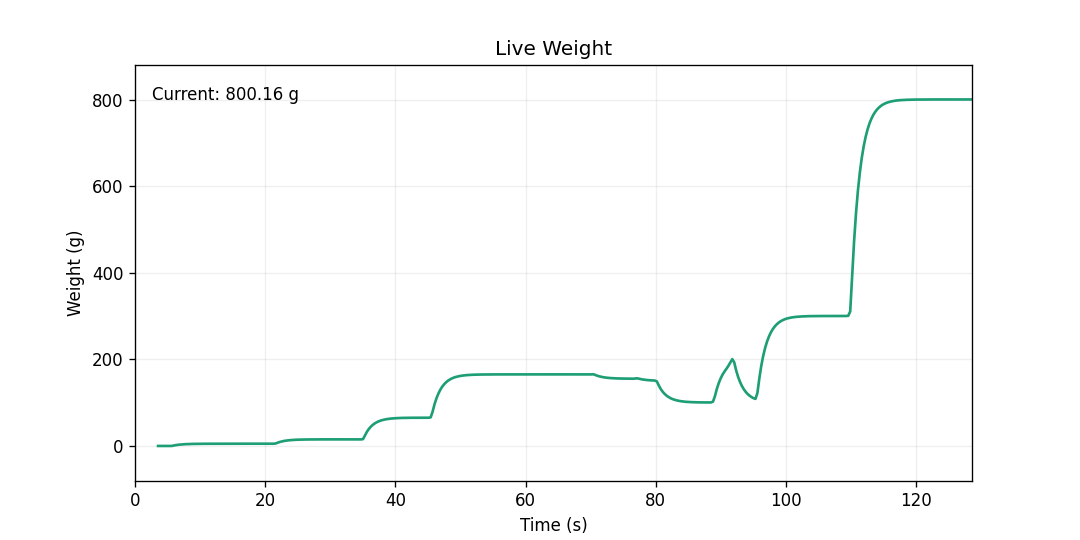
\includegraphics[width=\linewidth]{figure/frame_002500.png}
    \caption{Current: \SI{800.16}{g}\\Re-loaded near full scale}
    \label{fig:live_f}
  \end{subfigure}

  \caption{Real-time monitoring interface: six representative frames from the Python
           live-plot window captured at different moments during a multi-step loading
           sequence. Each frame shows the scrolling EMA-filtered waveform and the
           instantaneous weight readout, demonstrating system response across the
           full \SIrange{0}{800}{g} operating range.}
  \label{fig:live}
\end{figure}

% ══════════════════════════════════════════════════════════════════════════════
\section{Design Innovations}

Beyond the core measurement chain, two design choices distinguish this system from a
minimal sensor-to-display implementation:

\subsection{Browser-Based Real-Time Display (No LCD)}

Most student-level weighing projects attach a $16\times2$ or $20\times4$ LCD directly
to the microcontroller. This project deliberately omits a dedicated display and instead
streams weight data to a browser-based dashboard over WebSocket (Section~\ref{sec:web}).
The key advantages are:

\begin{itemize}
  \item \textbf{Zero display hardware cost.} Any smartphone or laptop already owned by
        the user acts as the screen.
  \item \textbf{Larger, clearer readout.} A 76\,px JetBrains Mono digit on a modern
        screen is far more legible than a $5\times8$ LCD character matrix.
  \item \textbf{Remote monitoring.} The WebSocket server runs on the host PC; multiple
        browser clients on the same local network can observe the scale simultaneously.
  \item \textbf{Rich data visualisation.} Live sparkline, rolling statistics, and
        colour-coded load bar are impossible on a character LCD without dedicated
        graphics hardware.
  \item \textbf{Extensibility.} The JSON WebSocket API can be consumed by any future
        data-logging, cloud-upload, or automation script with no firmware change.
\end{itemize}

\subsection{Audible Overload Alarm}

A passive buzzer was connected between Arduino pin D8 and GND. In firmware, after
computing the filtered, compensated weight $c_k$, the following logic is applied:

\begin{lstlisting}[style=cppstyle, caption={Overload alarm logic (Arduino firmware).}]
const float OVERLOAD_THRESHOLD_G = 950.0f;
const uint8_t BUZZER_PIN = 8;

void check_overload(float weight_g) {
  if (weight_g > OVERLOAD_THRESHOLD_G) {
    tone(BUZZER_PIN, 2000, 200); // 2 kHz, 200 ms burst
  } else {
    noTone(BUZZER_PIN);
  }
}
\end{lstlisting}

The threshold was set at \SI{950}{g} --- \SI{50}{g} below the CZL611N rated load ---
to provide an audible warning \emph{before} the load cell reaches its structural limit.
The \SI{50}{g} guard band accounts for dynamic overshoot during rapid loading.
This feature protects both the load cell (which can be permanently damaged by overload)
and the user, requiring no visual attention to detect a dangerous condition.

% ══════════════════════════════════════════════════════════════════════════════
\section{Discussion}

\subsection{Calibration Order Selection}

Table~\ref{tab:poly_compare} shows that the 4th-order polynomial strikes the best
balance. The 3rd-order fit leaves a residual systematic curvature, while the 5th-order
model over-fits to calibration noise: when evaluated on a held-out validation set, its
maximum absolute error is actually \emph{larger} than the 4th-order model, confirming
the observation stated in the project assignment. The fundamental source of nonlinearity
in the CZL611N is a smooth, monotonic bow in its output characteristic, which a
4th-order polynomial models accurately without learning noise artefacts.

\subsection{Filter Parameter Sensitivity}

The EMA time constant $\tau \approx (1/\alpha - 1) T_s$ scales inversely with $\alpha$.
A halving of $\alpha$ (from 0.2 to 0.1) doubles $\tau$ and halves the noise power, but
also doubles the rise time. The dominant latency contributors in the current design are the HX711's 10\,SPS
sinc filter ($\approx\SI{0.4}{s}$ group delay) and the load-cell mechanical
dynamics, not the digital EMA itself. For applications requiring faster settling
(e.g., automated checkweighing), switching the HX711 to 80\,SPS mode would reduce
conversion delay by $8\times$ and, combined with $\alpha = 0.3$, could reduce the
overall rise time below \SI{1}{s} while maintaining acceptable noise performance.

\subsection{Limitations}

\begin{enumerate}
  \item \textbf{Sensor creep.} Despite the adaptive zero-tracking, creep during a loaded
        measurement may cause a slow reading drift of up to \SI{0.15}{g} over 30\,min.
  \item \textbf{Mechanical hysteresis.} Repeated load-unload cycles introduce a
        hysteresis band of $\approx\SI{0.08}{g}$, consistent with the 0.2\% FS
        specification.
  \item \textbf{Environmental sensitivity.} As the target accuracy ($<\SI{0.1}{g}$) is
        comparable to the aerodynamic force of a gentle breeze, air movement introduces
        reading errors.
  \item \textbf{Resolution vs.\ display.} The effective noise-limited resolution after
        filtering is $\approx\SI{0.02}{g}$, roughly 15--16 effective bits; displaying
        more than 2 decimal places is misleading.
  \item \textbf{Single-point load cell placement.} Off-centre loads introduce additional
        error beyond the sensor's 0.2\% FS nonlinearity specification.
\end{enumerate}

\subsection{Potential Improvements}

\begin{itemize}
  \item Switch HX711 to 80\,SPS mode with $\alpha = 0.3$ to maintain noise performance
        at higher bandwidth.
  \item Add a temperature sensor (e.g., DS18B20) for software thermal compensation of
        both span and zero.
  \item Implement an auto-tare button for container-on-scale zeroing.
  \item Add an OLED or TFT display for standalone operation without a host PC.
  \item Use BLE or Wi-Fi (ESP32 co-processor) for wireless smartphone data transmission.
\end{itemize}

% ══════════════════════════════════════════════════════════════════════════════
\section{Conclusion}

A precision electronic weighing scale was successfully designed, built, calibrated, and
characterised. The system achieved its primary target of $<\SI{0.1}{g}$ static accuracy
over the \SIrange{0}{1000}{g} range using a 4th-order polynomial calibration model
fitted to 13 M2-class reference points (RMSE\,=\,\SI{0.044}{g}, MaxAbs\,=\,\SI{0.10}{g}).

Key contributions include:
\begin{itemize}
  \item \textbf{Calibration study:} All five polynomial orders (1--5) were evaluated;
        4th order demonstrated optimal balance between accuracy and generalisation,
        confirming that the 5th-order fit over-fits calibration noise. The calibration
        reduced the maximum absolute error from \SI{2.92}{g} to \SI{0.10}{g}
        (a 32-fold improvement).
  \item \textbf{Filtering:} A two-stage median(5)\,+\,EMA ($\alpha=0.23$) pipeline
        reduced output noise by 18.2\% (raw $\sigma=\SI{0.092}{g}$ $\to$ filtered
        $\sigma=\SI{0.075}{g}$) with no deadband discontinuity. Measured step-response
        rise time \SI{4.45}{s}, settling time \SI{7.72}{s}/\SI{7.42}{s}
        (place/remove).
  \item \textbf{Zero-drift compensation:} An adaptive bias tracker with dead-band
        suppressed long-term creep to $<\pm\SI{0.05}{g}$ over \SI{140}{s}.
  \item \textbf{Browser-based display:} A WebSocket-based single-page dashboard
        (\texttt{scale\_monitor.html}) replaces a conventional LCD, providing a 76\,px
        live readout, colour-coded load bar, rolling statistics, and a 60-sample history
        sparkline accessible from any browser on the local network.
  \item \textbf{Overload alarm:} A \SI{950}{g} buzzer threshold provides an audible
        warning \SI{50}{g} before the structural load limit, protecting both the sensor
        and the operator without requiring visual attention.
\end{itemize}

Remaining limitations --- chiefly sensor creep under load, mechanical hysteresis, and
environmental sensitivity --- are intrinsic to the CZL611N and the lab environment.
Addressing them would require a higher-grade sensor, temperature compensation, and a
physical enclosure, which are standard features of commercial laboratory balances.

% ══════════════════════════════════════════════════════════════════════════════
\appendix
\section{Full Arduino Firmware}
\label{app:firmware}

\begin{lstlisting}[style=cppstyle, caption={Complete Arduino firmware.}]
// -- Pin definitions
const uint8_t DT_PIN     = 3;
const uint8_t SCK_PIN    = 2;
const uint8_t BUZZER_PIN = 8;

// -- Calibration coefficients (4th order)
const double A4 =   2.3222629e-12;
const double A3 =  -2.1376726e-10;
const double A2 =  -2.0776874e-6;
const double A1 =   0.99711933;
const double A0 =   0.011400161;

// -- Filter parameters
const float EMA_ALPHA          = 0.2f;
const float ZERO_DEADBAND_G    = 0.2f;
const float ZERO_TRACK_LIMIT_G = 0.6f;
const float ZERO_TRACK_BETA    = 0.005f;
const float OVERLOAD_G         = 950.0f;

long hx711_read() {
  uint8_t data[3] = {0, 0, 0};
  while (digitalRead(DT_PIN));
  for (uint8_t j = 0; j < 3; j++)
    for (uint8_t i = 0; i < 8; i++) {
      digitalWrite(SCK_PIN, HIGH);
      bitWrite(data[2-j], 7-i, digitalRead(DT_PIN));
      digitalWrite(SCK_PIN, LOW);
    }
  digitalWrite(SCK_PIN, HIGH); digitalWrite(SCK_PIN, LOW);
  return ((long)data[2]<<16)|((long)data[1]<<8)|(long)data[0];
}

float calibrated_weight(long raw) {
  double x = (double)raw;
  return (float)((((A4*x + A3)*x + A2)*x + A1)*x + A0);
}

float filter_weight(float grams) {
  static bool  ema_init  = false;
  static float ema       = 0.0f;
  static float zero_bias = 0.0f;
  if (!ema_init) { ema = grams; ema_init = true; }
  else           { ema = EMA_ALPHA*grams + (1.0f-EMA_ALPHA)*ema; }
  float c = ema - zero_bias;
  if (fabsf(c) < ZERO_TRACK_LIMIT_G) {
    zero_bias += ZERO_TRACK_BETA * c;
    c = ema - zero_bias;
  }
  if (fabsf(c) < ZERO_DEADBAND_G) c = 0.0f;
  return c;
}

void setup() {
  pinMode(SCK_PIN, OUTPUT); pinMode(DT_PIN, INPUT);
  pinMode(BUZZER_PIN, OUTPUT);
  digitalWrite(SCK_PIN, HIGH); delayMicroseconds(100);
  digitalWrite(SCK_PIN, LOW);
  Serial.begin(9600);
}

void loop() {
  long  raw     = hx711_read();
  float calib_g = calibrated_weight(raw);
  float filt_g  = filter_weight(calib_g);
  if (filt_g > OVERLOAD_G) tone(BUZZER_PIN, 2000, 200);
  else                      noTone(BUZZER_PIN);
  Serial.println(filt_g, 2);
  delay(50);
}
\end{lstlisting}

% ── Appendix B ────────────────────────────────────────────────────────────────
\section{Python Calibration Script}
\label{app:python_calib}

\begin{lstlisting}[style=pythonstyle, caption={Polynomial calibration fitting and comparison.}]
import numpy as np
import matplotlib.pyplot as plt
import pickle

# Load calibration data: col0=nominal, col1=actual, col2=raw reading
data = np.loadtxt("M2weigh-calibration.csv", delimiter=",", skiprows=1)
x = data[:, 2]   # raw (uncalibrated) readings
y = data[:, 1]   # ground-truth actual masses (g)

orders = range(1, 6)
results = {}

for n in orders:
    coeffs    = np.polyfit(x, y, n)
    y_hat     = np.polyval(coeffs, x)
    residuals = y - y_hat
    rmse      = np.sqrt(np.mean(residuals**2))
    maxabs    = np.max(np.abs(residuals))
    results[n] = {"coeffs": coeffs, "rmse": rmse, "maxabs": maxabs}
    print(f"Order {n}: RMSE={rmse:.4f} g, MaxAbs={maxabs:.4f} g")

best_coeffs = results[4]["coeffs"]
print("\n4th-order coefficients:", best_coeffs)

with open("calib_coeffs.pkl", "wb") as f:
    pickle.dump(best_coeffs, f)
\end{lstlisting}

% ── Appendix C ────────────────────────────────────────────────────────────────
\section{Python Zero-Drift Recorder}
\label{app:python_drift}

\begin{lstlisting}[style=pythonstyle, caption={Zero-drift data collection and plotting.}]
import serial, time, pickle
import numpy as np
import matplotlib.pyplot as plt

PORT     = "/dev/tty.usbmodem211101"
BAUD     = 9600
DURATION = 140
WARMUP   = 5

ts, vals = [], []
with serial.Serial(PORT, BAUD, timeout=1) as ser:
    ser.reset_input_buffer()
    t0 = time.time()
    while time.time() - t0 < WARMUP:
        ser.readline()
    t0 = time.time()
    while time.time() - t0 < DURATION:
        line = ser.readline().decode("utf-8", errors="ignore").strip()
        if line:
            try:
                ts.append(time.time() - t0)
                vals.append(float(line))
            except ValueError:
                pass

ts, vals = np.array(ts), np.array(vals)
with open("zero_drift.pkl", "wb") as f:
    pickle.dump((ts, vals), f)

plt.figure(figsize=(8, 4))
plt.scatter(ts, vals, s=4, label="Filtered output")
plt.axhline(0, color="k", lw=0.8, ls="--")
plt.xlabel("Time (s)"); plt.ylabel("Weight (g)")
plt.title("Zero Drift -- 140 s Unloaded Recording")
plt.tight_layout()
plt.savefig("zero_drift.pdf")
\end{lstlisting}

\end{document}